\documentclass[a4paper,12pt,oneside]{article}

% ----- Header ----- %
\title{FPGA Development for the LHCb Vertex Locator Upgrade}
\author
{
	Nicholas Mead\\
	8064141\\
	School of Physics and Astronomy\\
	University of Manchester
}
\date{\today}

% ----- Packages ----- %
\usepackage[left=1in,right=1in,bottom=1.25in,top=1in]{geometry}
\usepackage{amsmath}
\numberwithin{equation}{section}
\numberwithin{figure}{section}
\numberwithin{table}{section}
\usepackage{graphicx}
\graphicspath{{Figures/}}
\usepackage{amsfonts}
\usepackage{bm}
\usepackage{enumerate}
\usepackage[ampersand]{easylist}
\usepackage{lineno}
\linenumbers
\modulolinenumbers[2]
\usepackage[backend=biber,sorting=none]{biblatex}
\addbibresource{Report_Main.bib}
\usepackage{placeins}
\let\Oldsection\section
\renewcommand{\section}{\FloatBarrier\Oldsection}
\let\Oldsubsection\subsection
\renewcommand{\subsection}{\FloatBarrier\Oldsubsection}
\let\Oldsubsubsection\subsubsection
\renewcommand{\subsubsection}{\FloatBarrier\Oldsubsubsection}
\usepackage{hhline} %double line for table

% ----- Settings ----- %	
\setlength{\parindent}{0em}
\setlength{\parskip}{1em}

% ----- Main ----- %
\begin{document}

	% ----- Document Head ----- %
	\begin{titlepage}
		\clearpage
		\maketitle \thispagestyle{empty}
		\vspace{1em}
		\begin{abstract}
	Lorem ipsum dolor sit amet, consectetur adipiscing elit. Curabitur blandit purus ut lacus aliquam, a sodales ante sodales. Etiam a elit nunc. Mauris ipsum tellus, ullamcorper et arcu at, cursus malesuada elit. In tempus pellentesque nisi, vel egestas enim cursus tempus. Sed velit urna, luctus sed efficitur sed, laoreet vitae magna. Mauris elementum dignissim lacus vitae tempus. Curabitur laoreet molestie dictum. Donec sit amet auctor nisl. \cite{LHCb}
	\\ \\
	Duis pellentesque euismod pellentesque. Praesent volutpat tincidunt eros, at faucibus tellus eleifend a. Quisque molestie sed ante sit amet sodales. Duis sed justo quam. Curabitur tellus felis, laoreet et bibendum a, posuere eget nisi. Donec suscipit lacinia porttitor. Aenean posuere sem nibh, et iaculis nisl faucibus eu. Donec ac posuere sapien. Aenean suscipit, nisi eget porttitor viverra, dui sapien vulputate lectus, ut dapibus purus orci nec arcu. Etiam placerat sapien non massa fringilla, et malesuada nibh hendrerit. Vestibulum et porttitor mi. Aliquam turpis velit, rutrum vitae erat at, scelerisque cursus lacus. Praesent libero urna, sodales efficitur eros id, sodales lacinia sem. Pellentesque habitant morbi tristique senectus et netus et malesuada fames ac turpis egestas.

\end{abstract}

		\newpage
		\thispagestyle{empty}	
		\tableofcontents
		\thispagestyle{empty}	
	
	\end{titlepage}

	% ----- Line Numbers for ease when writing ----- %
	% (comment out or remove for final draft) %
	\linenumbers
	\modulolinenumbers[2]

	% ----- Main Document ----- %

	\section{Introduction}

	\subsection{The Standard Model of Particle Physics}

    Central to the moden study of particle physics is the standard model,

    \begin{multline} \label{eqn:std-mod}
      L_{GWL} = \sum_{f} ( \bar{\Psi}_{f} ( i \gamma^\mu \partial \mu - m_{f} ) \Psi_{f} - eQ_{f} \bar{\Psi}_{f} \gamma^\mu \Psi_{f} A_{\mu} ) + \frac{g}{\sqrt{2}} \sum_{i} ( \bar{a}^i_L \gamma^\mu b^i_L W^+_\mu + \bar{b}^i_L \gamma^\mu a^i_L W^-_\mu )                        \\                           
              + \frac{g}{2x_w} \sum_f \bar{\Psi}_f \gamma^\mu ( I^3_f - 2s^2_w Q_f - I6e_f \gamma_5 ) \Psi_f Z_\mu - \frac{1}{4} | \partial_\mu A_v - \partial_v A_\mu - ie(W^-_\mu W^+_v - W^+_\mu W^-_v ) |^2                                         \\                                     
              - \frac{1}{2} | \partial_\mu W^+_v - \partial_v W^+_\mu - ie ( W^+_\mu A_v - W^+_v A_\mu ) + ig' c_w (W^+_\mu Z_v - W^+_v Z_\mu |^2 \\
              - \frac{1}{4} | \partial_\mu Z_v - \partial_v Z_\mu + ig' c_w (W^-_\mu W^+_v - W^+_\mu W^-_v ) |^2 - \frac{1}{2} M^2_\eta \eta^2  - \frac{gM^2_\eta}{8M_W} \eta^3  - \frac{g'^2 M^2_\eta}{32M_W}\eta^4    \\     
              + | M_W W^+_\mu + \frac{g}{2} \eta W^+_\mu |^2 + \frac{1}{2} | \partial_\mu \eta + i M_Z Z_\mu + \frac{ig}{2c_w} \eta Z_\mu |^2 - \sum_f \frac{g m_f}{2 M_W} \bar{\Psi}_f \Psi_f \eta.                                                                                
    \end{multline}

    The standard model, shown in equation \ref{eqn:std-mod}, is a quantum field theory that discribes the fundermental particles and how they interact.
    While this report does require, or attempt, a detailed understanding the intricate detail of the stardard model;
    the aim of many particle physics experiments is to varify, measure and expand the model.
    Dispite being the current best theory to explain particle interactions, the model is not complete.
    There are many undescribed phemomina, such as the matter domination in the universe, that require physics behond the standard model in order to be described.
    To that end, major international efforts, namely in the form of the Large Hardron Collider, aim to gain further knowledge and understanding of the underlying physics of the universe. \cite{ref:std}

  \subsection{Field Programable Gate Arrays}

  \subsection{The LHCb Experiment}

    One experiment at the Large Hadrom Colider is Large Hadron Colider beauty (LHCb).
    Located at intersection point 8, LHCb is designed to study rare particly physics phemonena, such as lepton flavour violation and CP violation. 
    The decays studied in the LCHb are via exotic hadronic decays of Bottom or Charm quarks that form sort lived hardons. 
    These hardons, commonly B mesons, travel in the order of a few cm in the detector before decaysing. As such, B meson decays can be identied by decay products that propogate via a secondary vertex.

    \begin{figure}[h!]
      \centering
      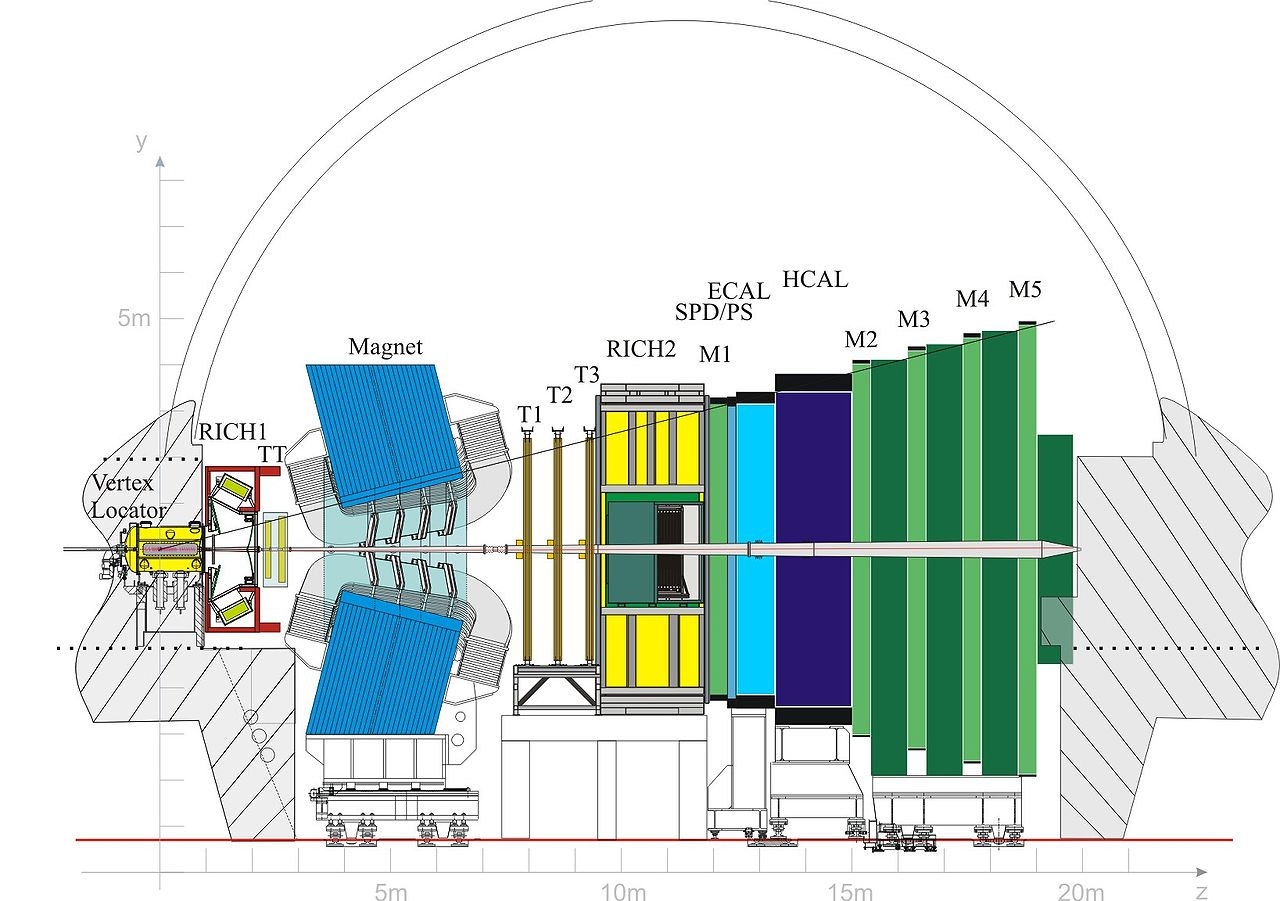
\includegraphics[scale=0.5]{LHCb_Det.jpg}
      \caption{The LHCb Detector along the bending plane.}
      \label{fig:LHCb_Collab}
    \end{figure}\FloatBarrier

    As B mesons are light (in comparision to other particles studied in the LHC), the decays products are produced at a shallow angle relivite the the beam pipe;
    this is the driving factor in the design of the exeperiment. 
    LHCb is a single arm forward spectormeter.
    Surrounding the point of collision is the \underline{Ve}rtex \underline{Lo}cator (VELO), this high precision detector uses silicon strips to detect ionising particles as they propogate from a collition and provides the coordinates of the particle in terms of R\footnote{Radial distance from the beam pipe.} and $\phi$\footnote{Asumthal angle.}.
    By reconstructing the paths of partics back to the intersection point, it can be identified wether or not the particular decay practicles are a product of the primary vertex\footnote{The position at which the protons collided.}, or a secondary vertex\footnote{The decay point of a short lived particle. i.e. B Meson.}.
    \par
    The Rich dectector, comprised of two subdectectors eitherside of the magnet, uses cherincov radiation to deduce the velocity of the particle. The silicon trackers, labeled TT and T1-3 in Figure~\ref{fig:LHCb_Collab}, calculate the angle deflection by the magnet. Be combining the velocity and angle of deflection, the mass, momentum and energy of the particles can be decuced from simple relitivistic kinematics.
    \par
    The meuon detectors, labeled M1-5 in Figure~\ref{fig:LHCb_Collab}, are important to detect muon's the detector. 
    This is of particular importance on LHCb as muons can be easily missidentified as charged pions, due to there simular mass.
    \par
    HCAl and ECAL, shown in Figure~\ref{fig:LHCb_Collab}, are hadronic and electric calorimeters respectively. 
    Both measure the total energy of incomming particles.
    As the calorimeters are absorbing of the particles they detect, any leptonic particle reaching the M2-5 muon detectors can be assumed to be a muon.
    Electrons and Photons are absorbed by the ECAl and any Tauons would have decayed long before reaching the far muon detectors.

      \subsection{LHCb Upgrade} % (fold)
      \label{sub:lhcb_upgrade}

      % subsection lhcb_upgrade (end)

      \subsubsection{VELO Upgrade}



      \subsubsection{The Role of FPGA's in the VELO Upgrade}

      


	\section{Scrambler}
\label{sec:scrambling_algorithms}

	Due to radiation levels inside the detector chamber, the main data processing takes place in a concrete bunker away from the detector.
	To facilitate this, 20 optical linkes (per modual) are used to transfer the data from the front end VELO to the Data Aquizition FPGA (DAQ).
	When comunicating data digitaly, the transfering modual (TX) and the recieving modual (RX) must have syncrinised clocks.
	In these case, the (name form dataflow) is the TX, and the DAQ is teh RX.
	When achieving syncronised close, there are two main approunches:

	\begin{easylist}
		\ListProperties(Numbers=R,Margin=0.5cm,Align=fixed,FinalSpace=2em)
		% & Syncinize both the TX and RX from a single central clock - used in I$^2$C communication.
		& Transmit the TX clock to the RX modual - used in I$^2$C and SPI communication.
		& Use bit-changes in the data to continuously synchronise the RX clock.
	\end{easylist}

	The former of these options, although the more convienient, is not appropriate for the VELO as it is suseptable to unforseens delays that could cause desyncronisation of the clocks to the data.
	The latter, while more invarient during delays, requires data with a high density of tranitions to reduce the likelyhood of a desyncronisation event.
	Becuase delays in the data are possible, the latter option has been selected.

	\subsection{The Role of Scrambling Data in the VELO}
		
		For the reasons described in Section \ref{sec:scrambling_algorithms}, it is nessesary to ensure that the data has large density of transitions before being transmitted from the front-end detector to the DAQ modual.
		However, as the majority of super pixel hitmaps are empty, the data has a bais towards \textit{`0'}s.
		This reduces the frequancy of transitions in the data - increasing the probability of a desyncronisation event.
		It is therefor nesseccary to scramble the data prior to transmition and descramble the data in the DAQ FPGA.
		\par
		Scrambling and later descrambling the data is not a trivial exercise.
		The scrambleing (TX) modual and descrambling (RX) modual must use a sycronised \textit{`key'}, that is used in both the scrambling and descrambling processes.
		In the FPGA, the \textit{`key'} is derived from the previous states of the data.
		There are two methods when generating this \textit{`key'}:

		\begin{description}
			\item[Additive] The \textit{`key'} is generated by evolving the previous \textit{`key'} at each itteration of data using the incoming frame.
			\item[Multiplicative] The  \textit{`key'} is generated from the previos $n$ frames. (Here $n$ is a variable specific to the algorithm).
		\end{description}



	\subsection{Scrambler Options}
	\label{sub:scrambler_options}

		Three scrambling algorithums have been concidered:

		\textbf{this section is out of date, but I dont have access to the uptoday section untill after I sent this. I have just not included it for now.}
		% \begin{description}
		% 	\item[Additive Scrambler] \hfill \\
		% 		This algoritum is simple and easy to use, however has the drawback of time dependance.
		% 		If a desyncronisation event occours, all subsequent data is rendered unrecoverable untill such time as a global reset signal is sent.
		% 		Further adding to the drawbacks, if a data packet is not sent from the TX during any clock cycle the RX descrambler will still evolve its descramble key - the TX sccrambler, however, will not.
		% 		This will ofcourse desyncronise the \textit{`keys'}, and as before all subsequent data is lost.

		% 	\item[Intermediate Scrambler] \hfill \\
		% 		Deriving its name from being the second algorithum under concideration, the Intermediate Scrambler is a \textbf{multiplicative} algorithm. 
		% 		The \textit{`key'} is generated from the current incoming frame and the previous frame.
		% 		Therefor, in the event of desyncronisation, only two frames are lost before the \textit{`key'} is automatically recovered.
		% 		This is a significant improvment over the Additive Scrambler.

		% 	\item[VeloPix Scrambler] \hfill \\
		% 		Named as, at the time of the start of the project \textit{(September 2015)}, this algorithum is the current preffered option by the VeloPix team; 
		% 		this too is a \textbf{multiplicative} algorithm.
		% 		The \textit{`key'} is, again like the Intermediate Scrambler, generaged from the currect and previous data frame.
		% 		The VeloPix Scrambler differse from the Intermediate scrambler as it aims to more effeciently scramble the data.
		% \end{description}


	\subsection{Cross Checks} % (fold)
	\label{sub:cross_checks}
	
		Ofcourse, the main prioritys when scrambling data is ensuring that the data in recoverable.
		For all three scramblers, the algorithum was sysnthesised in Quartus\cite{ref:quartus} and simulated in Modelsim\cite{ref:modelsim}.
		The aim of sysnthesising and simulating the scramblers in these programs was to ensure that the design was physical in term of on-board logic gates, and to check that the scrambled  data was recoverable.

		Furthermore, a C++ simulation was created for the three scramblers.
		This simulated had two purposes:
		firstly the output of the C++ can checked against the Modelsim simulated cehck consistancy;
		secondly to simulate the scrambler over a much larger simple of data as Modelsim simulations are less time effecient.
		In attition to the cross checks, the C++ code allowed for the injection of a desycronisation event.
		As expected, the additive scarmbler was unable to recover any data post-desycronisation, however the Intermediate and VeloPix scarmblers both recovered the \textit{`key'} after two frames and returned to descrambling data.

	% subsection cross_checks (end)

	\subsection{Algorithm Analysis}
	\label{sub:algorithm_analysis}

		One assumtion made is that fully scrambled data will be indistinguisable from randomly generated data. 
		For this reason, the three algorithm are not only tested against eachother and the pre-scrambled data but also randomly generated binary.
		The randomly generated data was created using the Python \textit{`random'} library, selecting a \textit{`0'} or \textit{`1'} with equal probubility.
		While the Python \textit{`random'} library is only sudo-random, on the scale of this example (i.e. $>$ 100,000 frames), it is by far sufficient.
		\par
		A more mathematically rigorous approuch, however, is to evaluate the system abstractly in the framework of statistical physics.
		In this abstraction, the 120 bit frame (with the header and parity removed) is concidered a ensemble; 
		microstates are the particular form of the frames;
		and macroscopic quantities can be calculated by averaging a large number of frames (i.e. the desync data).
		For the analysis outlined in section \ref{subsub:messurements_of_the_algorithms}, predictions will be made using these principles and outlined in section \ref{subsub:statistical_predictions}.
		\par
		In the context of the statisical model, it is reasonable to concider the degree of \textit{`scrambled-ness'} analogous to entropy.
		This analogy is not disimular to the common interpritation of entropy as a measure od dissorder.
		Therefor a scrambled system can be assumed to one of maximum entropy; and from Boltzmans law,

		\begin{equation}
			S \sim ln(\Omega)
			\label{eqn:boltzman}
		\end{equation}

		where $\Omega$ is the number of microstates assosiated with the macrostate, we learn that this state of maximum entropy is a macrostate with the maximum number of assosiated microstates.
		\par
		The entropic argument of Equation~\ref{eqn:boltzman} is not only mathematical founded.
		For a scramble algorithum to hold for all possible data sets, it must also be capable of outputing all possible permutations.
		As such, assuming all possible output are equally likely, the count of each macroscopic output will be proportional to the number of microstates assosiated.

		\subsubsection{Messurements of the Algorithms} 
		\label{subsub:messurements_of_the_algorithms}

			To compare the effecincy of the three algorithums in section \ref{sub:scrambler_options}, the algorithums where run over the same unput data and compared for the following measures:

			\begin{description}
				\item[Number of Transitions Per Frame] \hfill \\
					This meassure counts the total number of bit transitions (i.e. $bit(n) \neq bit(n-1)$) in a 120 bit frame. 
					The header and parity information was not included as they are not scrambled.
					This is an important test as one of the roles of the scrambler is to maximise the number of transitions.

				\item[Common Bit Chain Length] \hfill \\
					One of the downfalls of the `Number of Transitions Per Frame' analysis is that the two hypethetical 20 bit frames,

					\begin{enumerate}[a)]
						\item \textsc{10101010101111111111},
						\item \textsc{10011001100110011001},
					\end{enumerate}

					both with 10 transitions, are concidered equaly. However, (b) is clearly a more suitable output for data transfer as (a) has a large probability of desyncronisated due to the long chains of \textit{`1'}s in the right most bits.
					It is therefore also nessecary to evaluate the length of common bit chains within the scrambled data as shorter chains are more suitable for data transfer.

				\item[Bit Asymetry] \hfill \\
					Pre-scramble, the data had a large bais towards \textit{`0'}s due to the majority of the hitmaps being empty.
					Scrambled data, via entropic arguments, \textit{should} show zero bias eitherway.
					Therefor, by investigating how the inbalance of \textit{`1'}s and \textit{`0'}s evolves over many frames, any bias in the scrambler can be found.

			\end{description}	

		\subsubsection{Statistical Predictions} % (fold)
		\label{subsub:statistical_predictions}

			\begin{description}
				\item[Number of Transitions Per Frame] \hfill \\
					
					Consider a particle in a symmetric, descrete time-dependent, two state system,

					\begin{equation}
						p_0(t) = p_1(t) = 0.5, \quad : \quad \forall\ t \in \mathbb{N}
					\end{equation}

					at each time itteration,

					\begin{equation}
						p_{i \to j}(t) = 0.5. \quad : \quad i,j = [0\ 1], \quad \forall\ t \in \mathbb{N}
					\end{equation}

					However, assuming zero bias and detailed balance, as $p_{1 \to 0}(t)$ is equal in both probalility and importance to $p_{0 \to 1}(t)$, the probability of a bit change shall herefore be refered to as $p_{t}(t)$.
					\par
					Over a $n$ step process, analogous to a $n$ bit frame, the probalility distribution of the number of transitions $N_t$ is given by Binomial statistics,

					\begin{equation}
						f(N_{t}) = \frac{n!}{N_{t}!(n-N_{t})!}\ p^{N_{t}}\ (1 - p)^{n-N_{t}}
					\end{equation}

					Simplified for the special case $p = p_{t} = 0.5$,

					\begin{equation}
						f_{t}(N_{t}) = \frac{n!}{N_{t}!(n-N_{t})!}\ (p_{t})^{n}
						\label{eqn:transition_propability_dencity}
					\end{equation}

					For $n = 120$, we can calulate,

					\begin{equation}
						<N_t>^{Binomial} \ = \sum_{N_{t}=0}^{n-1} N_{t}\ f(N_{t}) = n\ p_{t} = 60
						\label{eqn:tansition_expectation}
					\end{equation}

					\begin{equation}
						\sigma_{N_t}^{Binomial} = \sqrt{ n\ p_{t}^2} = 5.48
					\end{equation}

					Furthermore, when concidering the entropic argument in section \ref{sub:algorithm_analysis} equation \ref{eqn:boltzman}, the number of microstates corespoding to each macrostate $N_t$ can be related to equation \ref{eqn:transition_propability_dencity},

					\begin{equation}
						\Omega_t = \binom{n}{N_t} = \frac{n!}{N_{t}!(n-N_{t})!}
					\end{equation}

					\begin{equation}
						<N_t>^{Entropic} = MAX[S_t] = MAX[\Omega_t]
					\end{equation}

					This can be numerically solved,

					\begin{equation}
						<N_t>^{Entropic}\ = 60
						\label{eqn:n_t_entropic}
					\end{equation}

					The result of equation \ref{eqn:n_t_entropic} is consistant with Equation~\ref{eqn:transitions_expectation}. This is an important as a \textit{`sanity check'} as the descrepincy would indicate an issue in the theory.

				\item[Common Bit Chain Length] \hfill \\
					
					The probability of a chain of length $n$ is,

					\begin{equation}
						p_n = p_1(1 - p_t)^{n-1}, \quad : \quad n \in \mathbb{N}, \quad n > 1
					\end{equation}

					where $p_1$ is the number of chains of lenght 1. 
					As $p_1 = N_0 (1 -p_t)$, where $N_0$ is the total number of chains,

					\begin{equation}
						\frac{N_n}{N_0} = (1 - p_t)^n, \quad : \quad n \in \mathbb{N}, \quad n > 1
					\end{equation}

					where $N_n$ in the number of chains of length $n$.
					Takeing the log of both sides,

					\begin{align}
						log\left(\frac{N_n}{N_0}\right) &= n\ log(1 - p_t), \nonumber \\
						log(N_n) &= n\  log(1 - p_t) + log(N_0).
					\end{align}

					Therefor, for a graph of $log(N_n)$ against $n$ for a large sample of data, the gradient would be $log(1 - p_t)$.
					In this case, as $p_t = 0.5$, 

					\begin{equation}
						log(1 - p_t) = -0.30\ .
						\label{eqn:log_chain_length_gradient}			
					\end{equation}

				\item[Bit Asymetry] \hfill \\
					
					$A_{1,0}$, the measure of assymetry of \textit{`1'}s and \textit{`0'}s is defined as,

					\begin{equation}
						A_{1,0} = N_1 - N_0,
						\label{eqn:a_def}
					\end{equation}

					where $N_1$ and $N_0$ are the number of \textit{`1'}s and \textit{`0'}s respectively.
					We can concider the evolution of $A_{1,0}$ with frame $t$ of size $n$ as a stockastic itterative map with zero deterministic growth \cite{ref:stockastic_physics},

					\begin{equation}
						A_{1,0}(nt + n\ \Delta t) = A_{1,0}(nt) + \mathcal{N}(nt)
					\end{equation}

					Where $\mathcal{N}$ is an independant random variable picked from a gausian distribution. While $A_{1,0}(t) \in \mathbb{Z}$, in the limit of large $nt$ we can approximate that $A_{1,0}$ is continious. 
					\par
					If we concider the moments of $A_{1,0}$,

					\begin{align}
						\label{eqn:A_moment1}
						<A_{1,0}(nt = M\ n\ \Delta t)> & = \sum_{m = 0}^{M -1}  \mathcal{N}(m\ n\ \Delta t), \\
						\label{eqn:A_moment2}
						<A_{1,0}(nt = M\ n\ \Delta t)^2> & = \sum_{m=0}^{M-1} \sum_{m'=0}^{M-1}  \mathcal{N}(m\ n\ \Delta t) \mathcal{N}(m'\ n\ \Delta t)\ \delta_{mm'} \nonumber \\
						&= \sum_{m=0}^{M-1} < \mathcal{N}(m\ n\ \Delta t)^2 >.
					\end{align}

					Clearly, in Equation \ref{eqn:A_moment1}, $<A> = 0$. In Equation \ref{eqn:A_moment2}, we assume the variance is of form $(\Delta t)^\alpha$ \cite{ref:stockastic_physics}. Then,

					\begin{equation}
						<A_{1,0}(nt = M\ \Delta t)^2>\ = M (n\ \Delta t)^\alpha.
						\label{eqn:A_moment3}
					\end{equation}

					Running the analysis over the frames $t = 0$ to $t_f$, the number of bits sampled is $M = {t_f / n\ \Delta t}$. Substituting this into Equation \ref{eqn:A_moment3},

					\begin{equation}
						<A_{1,0}(nt = M\ n\ \Delta t)^2>\ = t_f\ (n\ \Delta t)^{\alpha -1}.
					\end{equation}

					Concidering the three cases of $\alpha$ in the approximation of continious $n \Delta t$:
					\vspace{1em}
					\begin{easylist}[itemize]
						% \ListProperties{Margin=2cm,Align=fixed,FinalSpace=2em}
						& $\bm{\alpha > 1}$: Here $A_{1,0} \to 0$ as $n\ \Delta t \to 0$.
						& $\bm{\alpha < 1}$: Here $A_{1,0} \to \infty$ as $n\ \Delta t \to 0$.
						& $\bm{\alpha = 1}$: This is the only sensible choice.
					\end{easylist}
					\vspace{1em}
					With $\alpha =1$,

					\begin{equation}
						<A_{1,0}(nt = M\ n\ \Delta t)^2> = M (n\ \Delta t).
					\end{equation}

					And thus,

					\begin{equation}
						\sigma_{A_{1,0}} = \sqrt{<A_{1,0}^2> - <A_{1,0}>^2} = \sqrt{<A_{1,0}^2>} = \sqrt{n\ \Delta t}.
					\end{equation}

			\end{description}	

		\newpage
		\subsubsection{Results of Analysis}
		\label{subsub:alforithm_results}
			\vspace{-7mm}
			\begin{figure}[h]
				\centering
				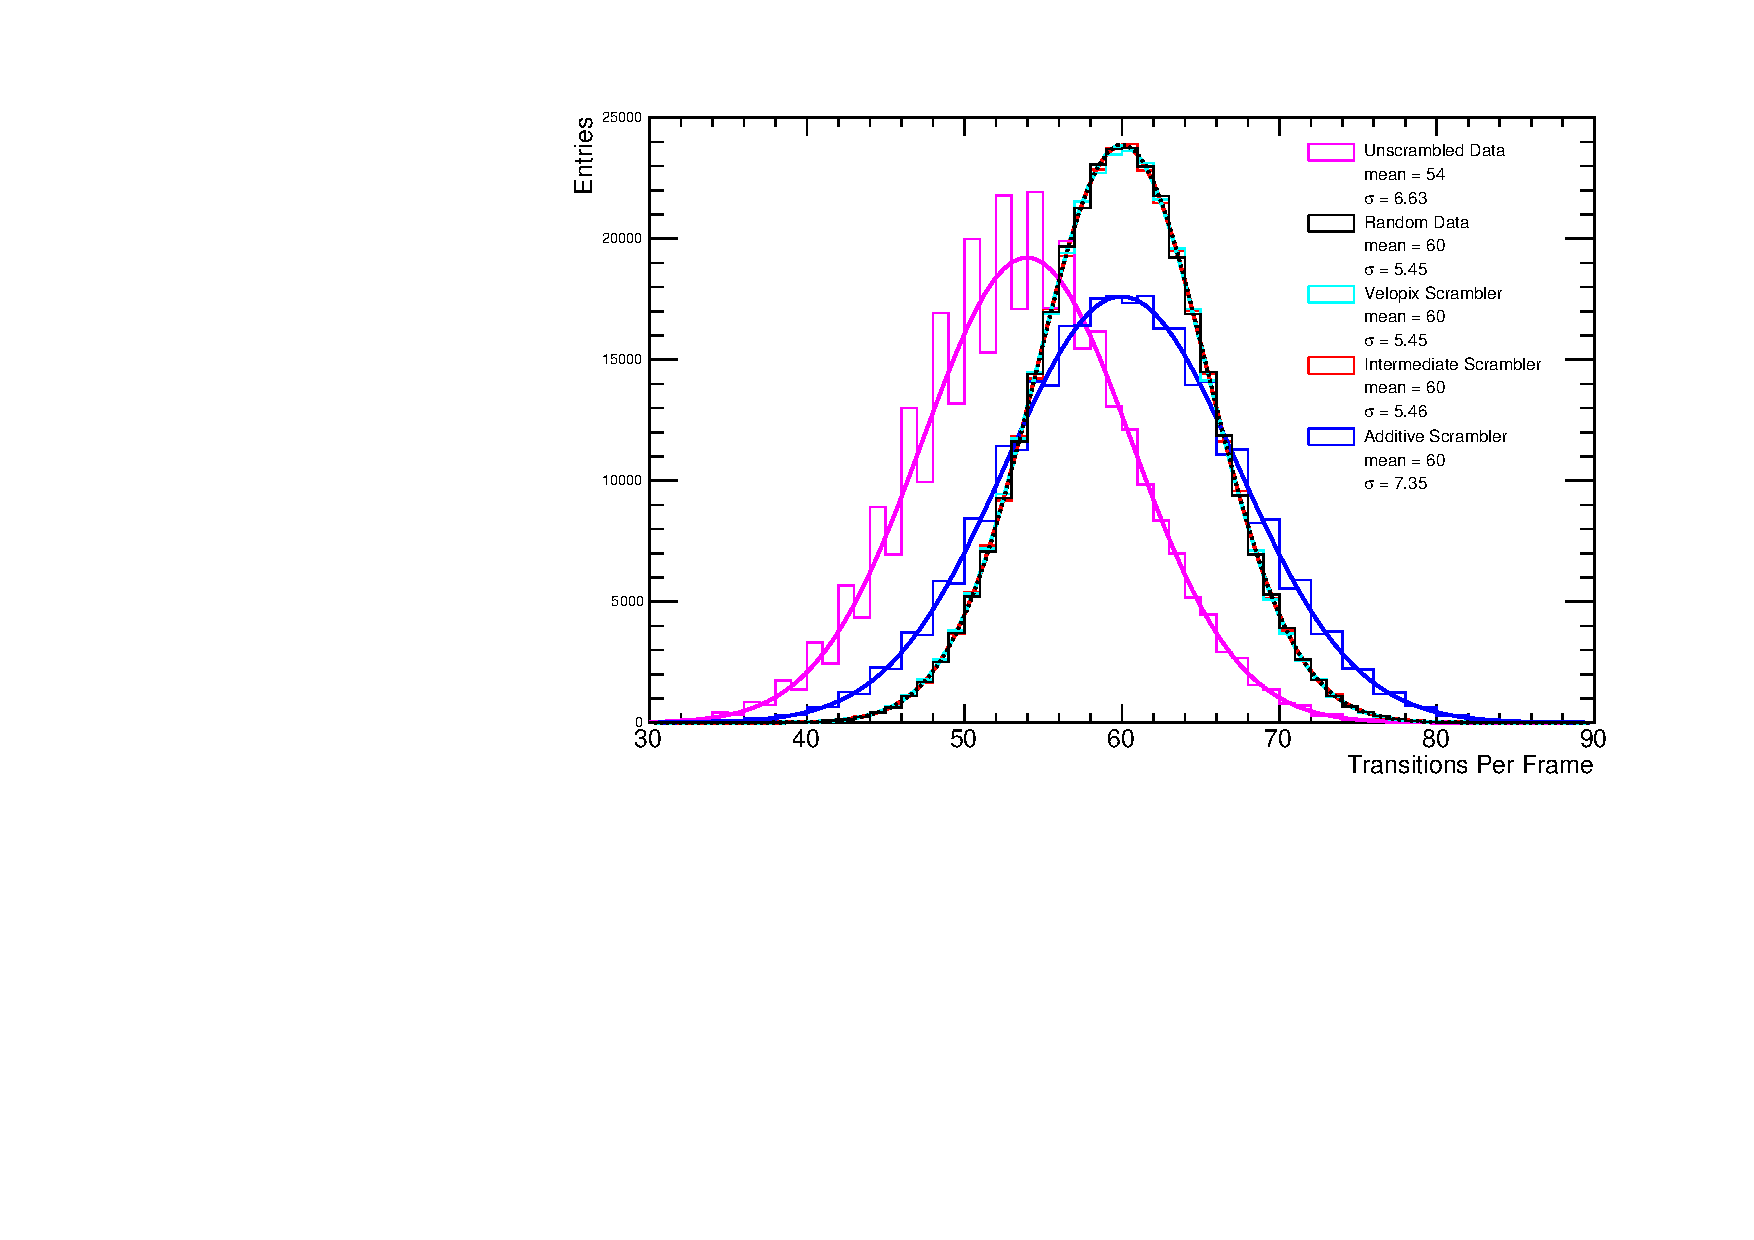
\includegraphics[width=0.75\textwidth]{Transition_Histogram_update}
				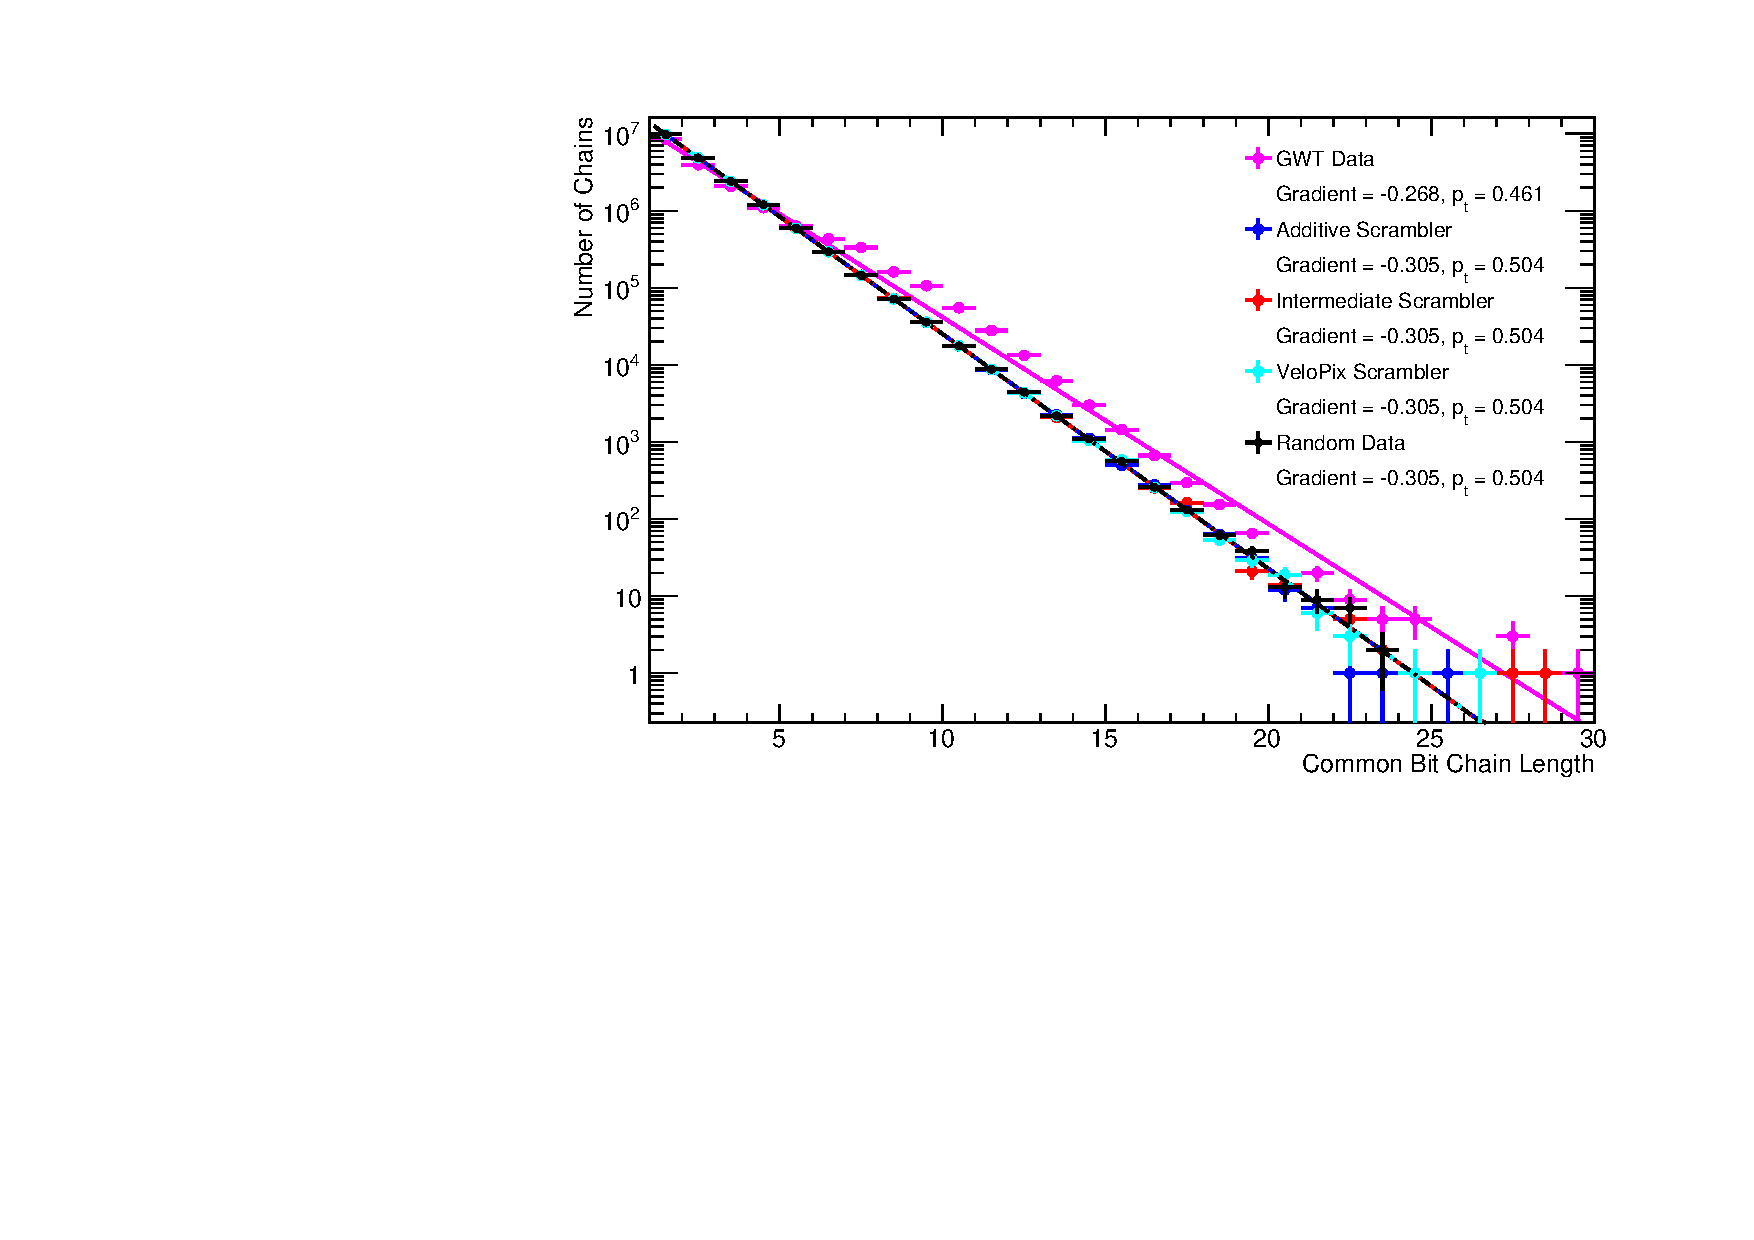
\includegraphics[width=0.75\textwidth]{Chain_length}
				\caption{Results of the \textit{`Number of Transitions Per Frame'} analysis (Top) and the \textit{`Common Bit Chain Length'} analysis (Bottom). The results for the Random Data, Intermediate Scrambler and VeloPix Scrambler overlap for the \textit{`Number of Transitions Per Frame'} analysis. The results for the Random Data, Additive Scrambler, Intermediate Scrambler and VeloPix Scrambler approximatly overlap for the \textit{`Common Bit Chain Length'} analysis.}
				\label{fig:transitions_per_frame}
			\end{figure} \FloatBarrier

			% \begin{figure}
			% 	\centering
			% 	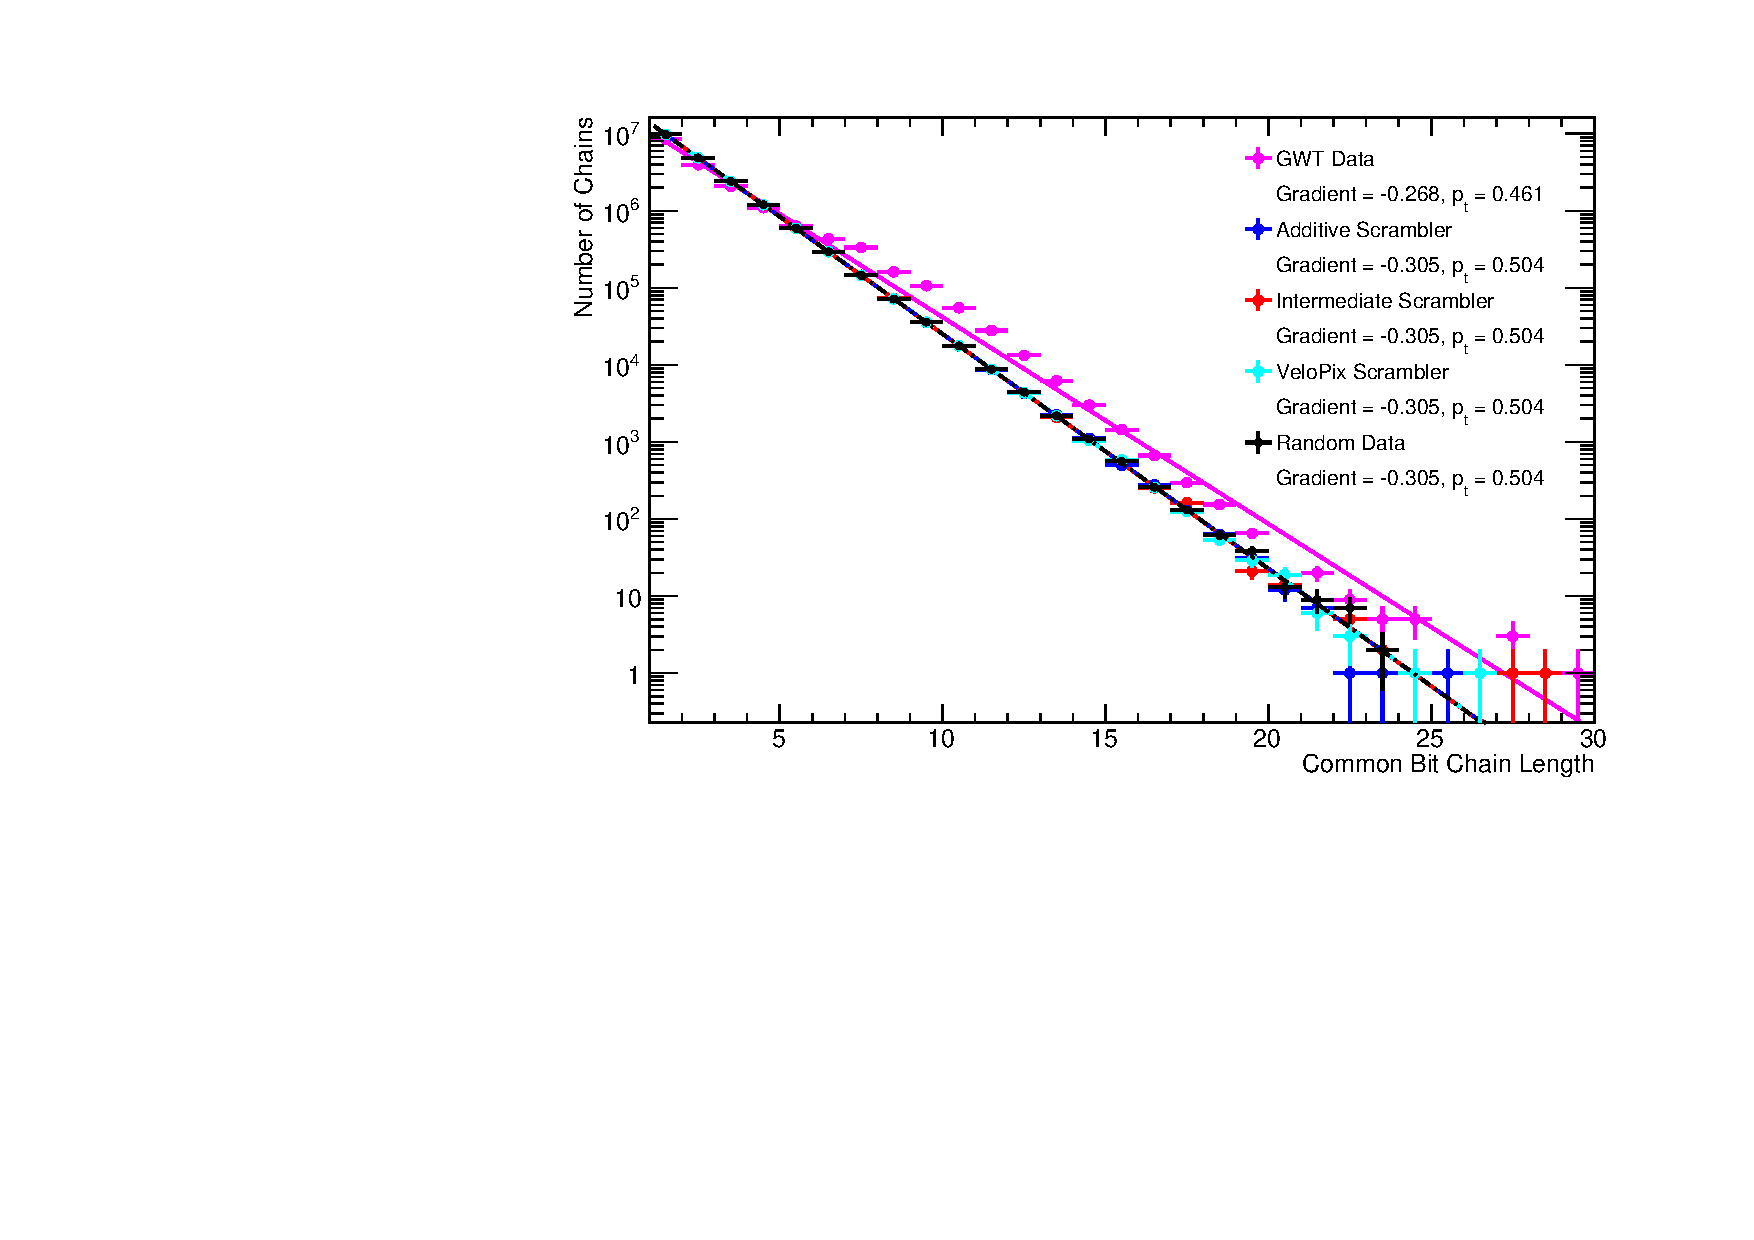
\includegraphics[width=0.75\textwidth]{Chain_length}
			% 	\caption{The results of the \textit{`Common Bit Chain Length'} analysis. The histograms and fits for the Random Data, Additive Scrambler, Intermediate Scrambler and VeloPix Scrambler approximatly overlap.}
			% 	\label{fig:chain_length}
			% \end{figure} \FloatBarrier
			
			The results from the \textit{`Number of Transitions Per Frame'} analysis, shown in Figure~\ref{fig:transitions_per_frame}, show a strong corelation between the Intermediate and VeloPix Scramblers with the randomly generated data. 
			These results are withing 1\% agreement with the theoretical predictions for $<N_t> = 60$ and $\sigma_{N_t} = 5.48$, made in Section~\ref{subsub:statistical_predictions}. 
			The remarkable consistancy between the theoretical predictions and the randomly gernerated data provides confidance in both the theory, and the scrambled nature of the Intermediate and VeloPix scrambler outputs.
			\par
			All three scramblers, the random data, and the theoretical predictions are all consistant to within 1\%. Comparing the two results for the Additive Scrambler, its shown that while the frequancy of longer chains is consistant with random data; but as the variance of transitions is larger than predicted, the long and short trains are more localy clustered. 

			% \begin{table}[h!]
			% 	\centering
			% 	\begin{TAB}(r,10cm)[5pt]{lcc}{c|c:ccc:cc}
					% 						& $<N_t>$	& $\sigma_{N_t}$ 	\\ %\hline
					% Unscrambled Data        & 54   		& 6.63     		\\ %\hdash
					% Additive Scrambler      & 60   		& 7.35     		\\
					% Intermediate Scrambler  & 60   		& 5.45     		\\
					% VeloPix Scrambler       & 60   		& 5.46     		\\ %\hdash
					% Random Data             & 60   		& 5.45     		\\
					% Theoretical Prediction  & 60   		& 5.48    		\\ 
			% 	\end{TAB}
			% 	\caption{The results of the \textit{`Number of Transitions Per Frame'} analysis.}
			% 	\label{tab:transitions_per_frame}
			% \end{table} 

			\begin{figure}
				\centering
				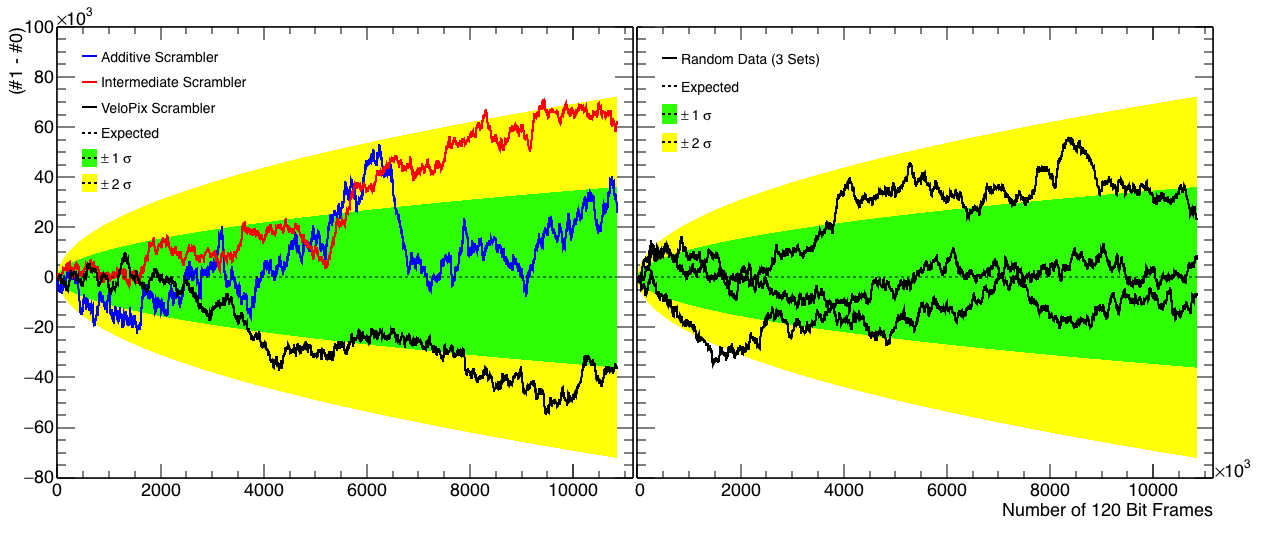
\includegraphics[width=1\textwidth]{Balance_graph_cropped}
				\caption{The results of the \textit{`Bit Asymetry'} analysis.}
				\label{fig:bit_asym}
			\end{figure}

			The \textit{`Bit Asymetry'} of each scrambler, shown in Figure~\ref{fig:bit_asym}, is consistant with the theoretical prediction. The deviation of $A_{1,0}$ for the predicted mean of 0 is fully consistant with stockastic noise. The random data also shows consistancy. This gives confidance in the assumtpions made in Section~\ref{subsub:statistical_predictions}.
			\par
			One notible feature of Figure\ref{fig:bit_asym} is the steap grandient of the additive scrambler a $t \sim 6.10^6$.
			However, as the data stays within the theoretical limits and the \textit{`drop'} is of approximatly $\Delta A_{1,0} \sim 60.10^3$ over the range $n\ \Delta t \sim 1.2.10^8$ it would be difficult to construnct any argument claiming that this feature is of statistically significance
			\par
			\textbf{(I am tempted to run $\chi^2$ analysis for a fit of y=0 so show that the data the data is consistant with the model, but am nut sure this will actually add to the argument?)}

			% \begin{table}[h!]
			% 	\centering
			% 	\begin{TAB}(r)[5pt]{lcc}{c|c:ccc:c}
					%              & Gradient  	& $p_t$    \\
					% Unscrambled  & -0.268 		& 0.460 \\
					% Additive     & -0.304 		& 0.504 \\
					% Intermediate & -0.304 		& 0.504 \\
					% Velopix      & -0.304 		& 0.504 \\
					% Random       & -0.304 		& 0.504 \\
			% 	\end{TAB}
			% 	\caption{The results of the \textit{`Common Bit Chain Length'} analysis.}
			% \end{table}

	\subsection{Conclusion}

		\begin{table}[h]
			\centering
			\begin{TAB}(r)[7pt]{l|cc:cc}{c|c:ccc:cc}
							           & $<N_t>$ & $\sigma_{N_t}$ & Gradient  	& $p_t$    \\
				GQT data  		       & 54      & 6.63           & -0.268 		& 0.460 \\
				Additive Scrambler     & 60      & 7.35           & -0.305 		& 0.504 \\
				Intermediate Scrambler & 60      & 5.45           & -0.305 		& 0.504 \\
				Velopix Scrambler      & 60      & 5.46           & -0.305 		& 0.504 \\
				Random Data            & 60      & 5.45           & -0.305 		& 0.504 \\
				Theoretical Prediction & 60      & 5.48           & -0.3    	& 0.5   	
			\end{TAB}
			\caption{The combined results of the algorithum analysis.}
			\label{tab:comb_results}
		\end{table}

		The consistancy of random data and the theoretical predictions justifies the assumptions and approximations made in Section~\ref{sub:algorithm_analysis} and Section~\ref{subsub:statistical_predictions}. Furthermore, the conformation of the statistical model allows for accurate comparisons to be made form predicted values and their measured counterparts.
		\par
		The Additive Scrambler, while consistant with the \textit{`Chain Length'} and \textit{`Bit Asymetry'} analysis, has a variance in the transition frequancy that leads the concultion that long and short chains are locally clusted. 
		This is not ideal for data transfer. 
		Many sequenchal long chains increase the probability of TX-RX clock desycronisation. 
		Furthermore, the additive scrambler will not recover from this loss of syncronisation, as the \textit{`key'} will never be recovered without a common reset signal.
		\par
		The Intermediate Scrambler produced an output consistant with random data. 
		This makes the algorithm suitable of data transfer.
		As already mentioned\footnote{Note to Marco: this is in the scrabler options section}, however, the scrambler is designed for computer simulated.
		As such, it is not suitable for implementation as it does not meet the additions requirments of the ASIC.
		\par
		The VeloPix Scrambler, like the Intermediate Scrambler, produces a statistically scrambled output.
		Furthermore, the algorithum in inline with the additional requirments of the ASIC.
		As such, it ideal for implementation, and hense is currently the choice algorithum for use in the 2019 VELO upgrade.











	\section{Event Isolation Flagging}
	
	\subsection{Motivation}

	\subsection{Time Sorting Data}

	\subsection{Bubble Sorting}

	\subsection{Isotation Checking}

	\subsection{Conclusion} 


	\section{Future Development}

	\subsection{LHCb 2020 Upgrade}

	\subsection{Further Development of FPGA's in the VELO}



	\section{Conclusion}

	This is the Conclusion

	% ----- Acknowledgements & Bibliography ----- %
	\section{Acknoledgments}
	I would like the Acknoledge Pablo Rodriguez and Marco Gersabeck for there continued support and supervision.


	\newpage 
	\addcontentsline{toc}{section}{References}
	\printbibliography

\end{document}
